% \documentclass[smaller, handout
% ]{beamer}
% % \usepackage{handoutWithNotes}
% % \pgfpagesuselayout{2 on 1 with notes}[letterpaper, landscape, border shrink=4mm]

\def\bmode{0} % Mode 0 for presentation, mode 1 for a handout with notes, mode 2 fo% r handout without notes
\if 0\bmode
\documentclass[smaller]{beamer}
\else \if 1\bmode
\immediate\write18{pdflatex -jobname=\jobname-Handout-Notes\space\jobname}
\documentclass[smaller,handout]{beamer}
\usepackage{handoutWithNotes}
\pgfpagesuselayout{2 on 1 with notes}[letterpaper, landscape, border shrink=4mm]
\else \if 2\bmode
\immediate\write18{pdflatex -jobname=\jobname-Handout\space\jobname}
\documentclass[smaller,handout]{beamer}
\fi
\fi
\fi

% \usepackage[T1]{fontenc} 
% \usepackage{lmodern} 
%\usepackage{etex}
 %\newcommand{\num}{6{} }

% \usetheme[
%   outer/progressbar=foot,
%   outer/numbering=fraction,
%   block=fill,
%   inner/subsectionpage=progressbar
% ]{metropolis}
\usetheme{Madrid}
\useoutertheme[subsection=false]{miniframes} % Alternatively: miniframes, infolines, split
\useinnertheme{circles}
% %\useoutertheme{Frankfurt}
% \usecolortheme{beaver}
% %\useoutertheme{crane}
% %\useoutertheme{metropolis}
\usepackage[backend=biber,style=authoryear,maxcitenames=2,maxbibnames=99,safeinputenc,url=false, eprint=false]{biblatex}
%\addbibresource{bib/references.bib}
% \AtEveryCitekey{\iffootnote{{\tiny}\tiny}{\tiny}}

% %\usepackage{pgfpages}
% %\setbeameroption{hide notes} % Only slides
% %\setbeameroption{show only notes} % Only notes
% %\setbeameroption{hide notes} % Only notes
% %\setbeameroption{show notes on second screen=right} % Both

% % \usepackage[sfdefault]{Fira Sans}

% % \setsansfont[BoldFont={Fira Sans}]{Fira Sans Light}
% % \setmonofont{Fira Mono}

% %\usepackage{fira}
% %\setsansfont{Fira}
% %\setmonofont{Fira Mono}
% % To give a presentation with the Skim reader (http://skim-app.sourceforge.net) on OSX so
% % that you see the notes on your laptop and the slides on the projector, do the following:
% % 
% % 1. Generate just the presentation (hide notes) and save to slides.pdf
% % 2. Generate onlt the notes (show only nodes) and save to notes.pdf
% % 3. With Skim open both slides.pdf and notes.pdf
% % 4. Click on slides.pdf to bring it to front.
% % 5. In Skim, under "View -> Presentation Option -> Synhcronized Noted Document"
% %    select notes.pdf.
% % 6. Now as you move around in slides.pdf the notes.pdf file will follow you.
% % 7. Arrange windows so that notes.pdf is in full screen mode on your laptop
% %    and slides.pdf is in presentation mode on the projector.

% % Give a slight yellow tint to the notes page
% \setbeamertemplate{note page}{\pagecolor{yellow!5}\insertnote}\usepackage{palatino}

% %\usetheme{metropolis}
% %\usecolortheme{beaver}
 \usepackage{tipa}
% \usepackage{enumerate}
% \definecolor{darkcandyapplered}{HTML}{A40000}
% \definecolor{lightcandyapplered}{HTML}{e74c3c}

% %\setbeamercolor{title}{fg=darkcandyapplered}

% \definecolor{UBCblue}{rgb}{0.04706, 0.13725, 0.26667} % UBC Blue (primary)
% \definecolor{UBCgrey}{rgb}{0.3686, 0.5255, 0.6235} % UBC Grey (secondary)

% % \setbeamercolor{palette primary}{bg=darkcandyapplered,fg=white}
% % \setbeamercolor{palette secondary}{bg=darkcandyapplered,fg=white}
% % \setbeamercolor{palette tertiary}{bg=darkcandyapplered,fg=white}
% % \setbeamercolor{palette quaternary}{bg=darkcandyapplered,fg=white}
% % \setbeamercolor{structure}{fg=darkcandyapplered} % itemize, enumerate, etc
% % \setbeamercolor{section in toc}{fg=darkcandyapplered} % TOC sections
% % \setbeamercolor{frametitle}{fg=darkcandyapplered,bg=white} % TOC sections
% % \setbeamercolor{title in head/foot}{bg=white,fg=white} % TOC sections
% % \setbeamercolor{button}{fg=darkcandyapplered} % TOC sections

% % % Override palette coloring with secondary
% % \setbeamercolor{subsection in head/foot}{bg=lightcandyapplered,fg=white}

%\usecolortheme{crane}
% \makeatletter
% \setbeamertemplate{headline}{%
%   \begin{beamercolorbox}[colsep=1.5pt]{upper separation line head}
%   \end{beamercolorbox}
%   \begin{beamercolorbox}{section in head/foot}
%     \vskip1pt\insertsectionnavigationhorizontal{\paperwidth}{}{}\vskip1pt
%   \end{beamercolorbox}%
%   \ifbeamer@theme@subsection%
%     \begin{beamercolorbox}[colsep=1.5pt]{middle separation line head}
%     \end{beamercolorbox}
%     \begin{beamercolorbox}[ht=2.5ex,dp=1.125ex,%
%       leftskip=.3cm,rightskip=.3cm plus1fil]{subsection in head/foot}
%       \usebeamerfont{subsection in head/foot}\insertsubsectionhead
%     \end{beamercolorbox}%
%   \fi%
%   \begin{beamercolorbox}[colsep=1.5pt]{lower separation line head}
%   \end{beamercolorbox}
% }
% \makeatother

% Reduce size of frame box
\setbeamertemplate{frametitle}{%
    \nointerlineskip%
    \begin{beamercolorbox}[wd=\paperwidth,ht=2.0ex,dp=0.6ex]{frametitle}
        \hspace*{1ex}\insertframetitle%
    \end{beamercolorbox}%
}


%\setbeamercolor{frametitle}{bg=darkcandyapplered!80!black!90!white}
%\setbeamertemplate{frametitle}{\bf\insertframetitle}

%\setbeamercolor{footnote mark}{fg=darkcandyapplered}
%\setbeamercolor{footnote}{fg=darkcandyapplered!70}
%\Raggedbottom
%\setbeamerfont{page number in head/foot}{size=\tiny}
%\usepackage[tracking]{microtype}


% %\usepackage[sc,osf]{mathpazo}   % With old-style figures and real smallcaps.
% %\linespread{1.025}              % Palatino leads a little more leading

% % Euler for math and numbers
% %\usepackage[euler-digits,small]{eulervm}
% %\AtBeginDocument{\renewcommand{\hbar}{\hslash}}
\usepackage{graphicx,multirow,booktabs}


% %\mode<presentation> { \setbeamercovered{transparent} }

\setbeamertemplate{navigation symbols}{}
\makeatletter
\def\beamerorig@set@color{%
  \pdfliteral{\current@color}%
  \aftergroup\reset@color
}
\def\beamerorig@reset@color{\pdfliteral{\current@color}}
\makeatother


% %=== GRAPHICS PATH ===========
\graphicspath{{./images/}}
% % Marginpar width
% %Marginpar width
% %\setlength{\marginparsep}{.02in}


% %% Captions
% % \usepackage{caption}
% % \captionsetup{
% %   labelsep=quad,
% %   justification=raggedright,
% %   labelfont=sc
% % }

% \setbeamerfont{caption}{size=\footnotesize}
% \setbeamercolor{caption name}{fg=darkcandyapplered}

% %AMS-TeX packages

\usepackage{amssymb,amsmath,amsthm,mathtools} 
\usepackage{bm}
% \usepackage{color}

% %https://tex.stackexchange.com/a/31370/2269
% \usepackage{mathtools,cancel}

% \renewcommand{\CancelColor}{\color{red}} %change cancel color to red

% \makeatletter
% \let\my@cancelto\cancelto %copy over the original cancelto command
% \newcommand<>{\cancelto}[2]{\alt#3{\my@cancelto{#1}{#2}}{\mathrlap{#2}\phantom{\my@cancelto{#1}{#2}}}}
% % redefine the cancelto command, using \phantom to assure that the
% % result doesn't wiggle up and down with and without the arrow
% \makeatother


% %\usepackage{comment}
% %\usepackage{hyperref,enumerate}
% \usepackage{minitoc,array}

% \definecolor{slblue}{rgb}{0,.3,.62}
% % \hypersetup{
% %     colorlinks,%
% %     citecolor=blue,%
% %     filecolor=blue,%
% %     linkcolor=blue,
% %     urlcolor=slblue
% % }

% \usepackage{epstopdf}
% \epstopdfDeclareGraphicsRule{.gif}{png}{.png}{convert gif:#1 png:\OutputFile}
% \AppendGraphicsExtensions{.gif}

% %\usepackage{listings}

% %%% TIKZ
% \usepackage{forest}
\usepackage{tikz}
\usepackage{pgfplots}
\usepackage{pgfplotstable}
%\usepackage{pgfgantt}
\pgfplotsset{compat=newest}

\usetikzlibrary{fit,arrows,shapes,positioning,shapes.geometric}
\usetikzlibrary{decorations.markings}
\usetikzlibrary{shadows,automata}
\usetikzlibrary{patterns}
\usetikzlibrary{trees,mindmap,backgrounds}
%\usetikzlibrary{circuits.ee.IEC}
\usetikzlibrary{decorations.text}
% % For Sagnac Picture
% \usetikzlibrary{%
%     decorations.pathreplacing,%
%     decorations.pathmorphing%
% }
% \tikzset{no shadows/.style={general shadow/.style=}}
% %
% %\usepackage{paralist}

% \tikzset{
%   font=\Large\sffamily\bfseries,
%   red arrow/.style={
%     midway,red,sloped,fill, minimum height=3cm, single arrow, single arrow head extend=.5cm, single arrow head indent=.25cm,xscale=0.3,yscale=0.15,
%     allow upside down
%   },
%   black arrow/.style 2 args={-stealth, shorten >=#1, shorten <=#2},
%   black arrow/.default={1mm}{1mm},
%   tree box/.style={draw, rounded corners, inner sep=1em},
%   node box/.style={white, draw=black, text=black, rectangle, rounded corners},
% }

% %%% FORMAT PYTHON CODE
% %\usepackage{listings}
% % Default fixed font does not support bold face
% \DeclareFixedFont{\ttb}{T1}{txtt}{bx}{n}{8} % for bold
% \DeclareFixedFont{\ttm}{T1}{txtt}{m}{n}{8}  % for normal

% % Custom colors
% \definecolor{deepblue}{rgb}{0,0,0.5}
% \definecolor{deepred}{rgb}{0.6,0,0}
% \definecolor{deepgreen}{rgb}{0,0.5,0}

% %\usepackage{animate}

% % Python style for highlighting
% % \newcommand\pythonstyle{\lstset{
% % language=Python,
% % basicstyle=\footnotesize\ttm,
% % otherkeywords={self},             % Add keywords here
% % keywordstyle=\footnotesize\ttb\color{deepblue},
% % emph={MyClass,__init__},          % Custom highlighting
% % emphstyle=\footnotesize\ttb\color{deepred},    % Custom highlighting style
% % stringstyle=\color{deepgreen},
% % frame=tb,                         % Any extra options here
%     % showstringspaces=false            % 
% % }}

% % % Python environment
% % \lstnewenvironment{python}[1][]
% % {
% % \pythonstyle
% % \lstset{#1}
% % }
% % {}

% % % Python for external files
% % \newcommand\pythonexternal[2][]{{
% % \pythonstyle
% % \lstinputlisting[#1]{#2}}}

% % Python for inline
% % 
% % \newcommand\pythoninline[1]{{\pythonstyle\lstinline!#1!}}

% %\usepackage{algorithm2e}

\newcommand{\eps}{\epsilon}
\newcommand{\bX}{\mb X}
\newcommand{\by}{\mb y}
\newcommand{\bbe}{\bm\beta}
\newcommand{\beps}{\bm\epsilon}
\newcommand{\bY}{\mb Y}

\newcommand{\osn}{\oldstylenums}
\newcommand{\dg}{^{\circ}}
\newcommand{\lt}{\left}
\newcommand{\rt}{\right}
\newcommand{\pt}{\phantom}
\newcommand{\tf}{\therefore}
\newcommand{\?}{\stackrel{?}{=}}
\newcommand{\fr}{\frac}
\newcommand{\dfr}{\dfrac}
\newcommand{\ul}{\underline}
\newcommand{\tn}{\tabularnewline}
\newcommand{\nl}{\newline}
\newcommand\relph[1]{\mathrel{\phantom{#1}}}
\newcommand{\cm}{\checkmark}
\newcommand{\ol}{\overline}
\newcommand{\rd}{\color{red}}
\newcommand{\bl}{\color{blue}}
\newcommand{\pl}{\color{purple}}
\newcommand{\og}{\color{orange!90!black}}
\newcommand{\gr}{\color{green!40!black}}
\newcommand{\dca}{\color{darkcandyapplered}}
\newcommand{\nin}{\noindent}
\newcommand*\circled[1]{\tikz[baseline=(char.base)]{
            \node[shape=circle,draw,thick,inner sep=1pt] (char) {\small #1};}}

\newcommand{\bc}{\begin{compactenum}[\quad--]}
\newcommand{\ec}{\end{compactenum}}

\newcommand{\p}{\partial}
\newcommand{\pd}[2]{\frac{\partial{#1}}{\partial{#2}}}
\newcommand{\dpd}[2]{\dfrac{\partial{#1}}{\partial{#2}}}
\newcommand{\pdd}[2]{\frac{\partial^2{#1}}{\partial{#2}^2}}
\newcommand{\pde}[3]{\frac{\partial^2{#1}}{\partial{#2}\partial{#3}}}
\newcommand{\nmfr}[3]{\Phi\left(\frac{{#1} - {#2}}{#3}\right)}
\newcommand{\Err}{\text{Err}}
\newcommand{\err}{\text{err}}

%\DeclarePairedDelimiter\ceil{\lceil}{\rceil}
%\DeclarePairedDelimiter\floor{\lfloor}{\rfloor}

%%%% GREEK LETTER SHORTCUTS %%%%%
\newcommand{\la}{\lambda}
\renewcommand{\th}{\theta}
\newcommand{\al}{\alpha}
\newcommand{\G}{\Gamma}
\newcommand{\si}{\sigma}
\newcommand{\Si}{\Sigma}


\pgfmathdeclarefunction{poiss}{1}{%
  \pgfmathparse{(#1^x)*exp(-#1)/(x!)}%
  }

\pgfmathdeclarefunction{gauss}{2}{%
  \pgfmathparse{1/(#2*sqrt(2*pi))*exp(-((x-#1)^2)/(2*#2^2))}%
}

\pgfmathdeclarefunction{expo}{2}{%
  \pgfmathparse{#1*exp(-#1*#2)}%
}

\pgfmathdeclarefunction{expocdf}{2}{%
  \pgfmathparse{1 -exp(-#1*#2)}%
}

\newcommand{\ldate}{Feb 16, 2025}
\newcommand{\mb}{\mathbb}
\newcommand{\mc}{\mathcal}
\newcommand{\tr}{^{\top}}
% \usepackage{pst-plot}

% \usepackage{pstricks-add}
% \usepackage{auto-pst-pdf}   

% \psset{unit = 3}

% \def\target(#1,#2){%
%  {\psset{fillstyle = solid}
%   \rput(#1,#2){%
%     \pscircle[fillcolor = white](0.7,0.7){0.7}
%     \pscircle[fillcolor = blue!60](0.7,0.7){0.5}
%     \pscircle[fillcolor = white](0.7,0.7){0.3}
%     \pscircle[fillcolor = red!80](0.7,0.7){0.1}}}}
% \def\dots[#1](#2,#3){%
%     \psRandom[
%       dotsize = 2pt,
%       randomPoints = 25
%     ](!#2 #1 0.04 sub sub #3 #1 0.04 sub sub)%
%      (!#2 #1 0.04 sub add #3 #1 0.04 sub add)%
%      {\pscircle[linestyle = none](#2,#3){#1}}}


%%%%%%%%%%%%%%%%%%%%%%%%%%%%%%%%%%%%%%%%%%%%%%%%%%%
%%%%%%%%%%%%%%%%%%%%%%%%%%%%%%%%%%%%%%%%%%%%%%%%%%%
\title[CEE 616 1e: Linear Algebra]{ {\normalsize CEE 616:  Probabilistic Machine Learning}
  \\ Lecture 1e: Foundations---Linear Algera}
\date[\ldate]{\footnotesize \ldate}
\author{{\bf Jimi Oke}}
\institute[UMass Amherst]{
%\titlegraphic{\hfill
  \begin{tikzpicture}[baseline=(current bounding box.center)]
    \node[anchor=base] at (-7,0) (its) {
\includegraphics[scale=.3]{UMassEngineering_vert}} ;
  \end{tikzpicture}
  % \hfill\includegraphics[height=1.5cm]{logo}
}

%https://tex.stackexchange.com/questions/55806/mindmap-tikzpicture-in-beamer-reveal-step-by-step
  \tikzset{
    invisible/.style={opacity=0},
    visible on/.style={alt={#1{}{invisible}}},
    alt/.code args={<#1>#2#3}{%
      \alt<#1>{\pgfkeysalso{#2}}{\pgfkeysalso{#3}} % \pgfkeysalso doesn't change the path
    },
  }


% https://tex.stackexchange.com/questions/446468/labels-with-arrows-for-an-equation
% https://tex.stackexchange.com/a/402466/121799
\newcommand{\tikzmark}[3][]{
\ifmmode
\tikz[remember picture,baseline=(#2.base)] \node [inner sep=0pt,#1](#2) {$#3$};
\else
\tikz[remember picture,baseline=(#2.base)] \node [inner sep=0pt,#1](#2) {#3};
\fi
}

% \lstset{language=matlab,
%                 basicstyle=\scriptsize\ttfamily,
%                 keywordstyle=\color{blue}\ttfamily,
%                 stringstyle=\color{blue}\ttfamily,
%                 commentstyle=\color{gray}\ttfamily,
%                 morecomment=[l][\color{gray}]{\#}
%               }


              
\begin{document}

\maketitle

\begin{frame}
  \frametitle{Outline}
  \tableofcontents
\end{frame}

\section{Inroduction}
\begin{frame}
  \frametitle{Scalars, vectors and matrices}\pause
  \begin{itemize}
  \item \textbf{Scalar:} a single number, e.g \pause $a \in \mathbb{R}$\pause
  \item \textbf{Vector:} ordered array of numbers, e.g.\pause $\bm x
    \in \mb{R}^n$ \pause
    \begin{equation*}
      \bm{x} = \begin{bmatrix} x_{1}\\ x_{2}\\ \vdots\\ x_{n} \end{bmatrix}
    \end{equation*}\pause
  \item \textbf{Matrix:} two-dimensional array of numbers, e.g. $\bm X \in \mathbb{R}^{n\times p} $
    \pause
    \begin{equation*}
      \bm X =
      \begin{bmatrix}
        x_{11} & x_{12} & \cdots & x_{1p} \\
        x_{21} & x_{22} & \cdots & x_{2p} \\
        \vdots & \vdots & \ddots & \vdots \\
        x_{n1} & x_{n2} & \cdots & x_{np} \\        
      \end{bmatrix}
    \end{equation*}
    \pause
    Each element $x_{ij} = [\bm X]_{ij}\in \mathbb{R}, \pause \forall i \in \{1:n\}, j \in \{1:p\}$
    
  \end{itemize}

\end{frame}


\begin{frame}
  \frametitle{Tensors}

  \begin{itemize}
  \item \textbf{Tensor:} generalization of a matrix to arbitrary
    number of indices/dimensions, e.g.\ 3 ($x_{ijk}$)

    \pause

  \item Number of dimensions is called \textbf{order}/\textbf{rank}
    \pause

  \item A common application is the representation of an RGB image,
    e.g.\ a square 256-pixel image can be denoted by $\bm A\in \mb
    R^{256\times 256\times 3}$

  \end{itemize}
\end{frame}





\begin{frame}
  \frametitle{Vector and matrix multiplication}
  \pause

  \begin{block}{Dot/inner product of two vectors}
    \pause
    \begin{equation}
      \bm x\cdot\bm y = \pause \bm x\tr \bm y = \pause
      \begin{bmatrix}
        x_{1} & \cdots & x_{N} 
      \end{bmatrix}
      \times
      \begin{bmatrix}
        y_{1} \\ \vdots \\ y_{N}
      \end{bmatrix}
      \pause = \sum_{n=1}^{N} x_{n}y_{n}
    \end{equation}
  \end{block}
  \pause
  \begin{block}{Matrix product}
    \pause
    \begin{equation}
      \bm A_{M\times N} \bm B_{N\times D} = \pause \bm C_{M\times D}
    \end{equation}
    \pause
    Each element $[\bm C]_{md}$ is obtained as the dot product between the $m$th row of $\bm A$ and the $d$-th column of $\bm B$.
  \end{block}
\end{frame}

\begin{frame}
  \frametitle{Matrix multiplication properties}
  \pause
  \begin{itemize}[<+->]
  \item Distributivity \pause
    \begin{equation}
      \bm A(\bm B + \bm C) = \pause \bm{AB} + \bm{AC}
    \end{equation}
    \pause
  \item Associativity \pause
    \begin{equation}
    \bm A(\bm{BC}) = \pause (\bm{AB})\bm C
  \end{equation}
  \pause

\item Conjugate transposability \pause
  \begin{equation}
    (\bm{AB})\tr = {\bm B\tr\bm A\tr}
  \end{equation}
  
\end{itemize}
\pause

\begin{alertblock}{Non-commutativity}
  Unlike the inner product of two vectors, where $\bm x\tr\bm y = \bm y\tr\bm x$, \pause
  matrix multiplication is not commutative:\pause
  \begin{equation}
    \bm{AB} \ne \bm{BA}
  \end{equation}
\end{alertblock}
\end{frame}


\section{Vectors}



\begin{frame}
	\frametitle{Linear independence}
	
	\pause
	
	A set of vectors $\{\bm x_1, \bm x_2, \ldots, \bm x_n\}$ is said to
	be linearly independent (LI) if no vector in the set can be
	expressed as a linear combination of the others.
	\pause
	
	\begin{itemize}
		\item If a vector $\bm x_j$ in the set can be written as:
		\pause
		\begin{equation}
			\bm x_j = \sum_{i\ne j}^n \alpha_i \bm x_i
		\end{equation}
		Then $\bm x_j$ is dependent on the others, so the set is not LI
		\pause
		
		\item Another way to view this:
		\pause
		\begin{equation}
			\nexists \bm \alpha \in \mb{R}^n \quad \text{s.t.}\quad \alpha_1\bm x_1 +
			\cdots + \alpha_n\bm x_n = \bm 0
		\end{equation}
		
	\end{itemize}
	
\end{frame}

\begin{frame}
	\frametitle{Span}
	\pause
	The \textbf{span} of a set of vectors $\{\bm x_1, \bm x_2, \ldots, \bm x_n\}$
	is the set of all vectors that can be expressed as a linear
	combination of the set: \pause
	\begin{equation}
		\text{span}( \{\bm x_1, \bm x_2, \ldots, \bm x_n\}) := \pause
		\lt\{ \bm v : \bm v = \sum_{i=1}^n \alpha_i\bm x_i,\quad \alpha_i
		\in \mb{R}\rt\}
	\end{equation}
	
	\pause
	\begin{alertblock}{Result}
		If a set of vectors is LI, then any vector $\bm v \in \mb{R}^n$
		can be written as a linear combination of $\bm x_1$ through
		$\bm x_n$
	\end{alertblock}
	\pause
	
\end{frame}

\begin{frame}
	\frametitle{Basis}
	A set of LI vectors that span an entire vector space $\mc{V}$ is
	called a \textbf{basis} $\mc{B}$.
	\pause
	\begin{itemize}
		\item Every element of $\bm v\in \mc{V}$ can be expressed as a
		linear combination of corresponding elements in $\mc{B}$.
	\end{itemize}
	\pause
	\begin{center}
		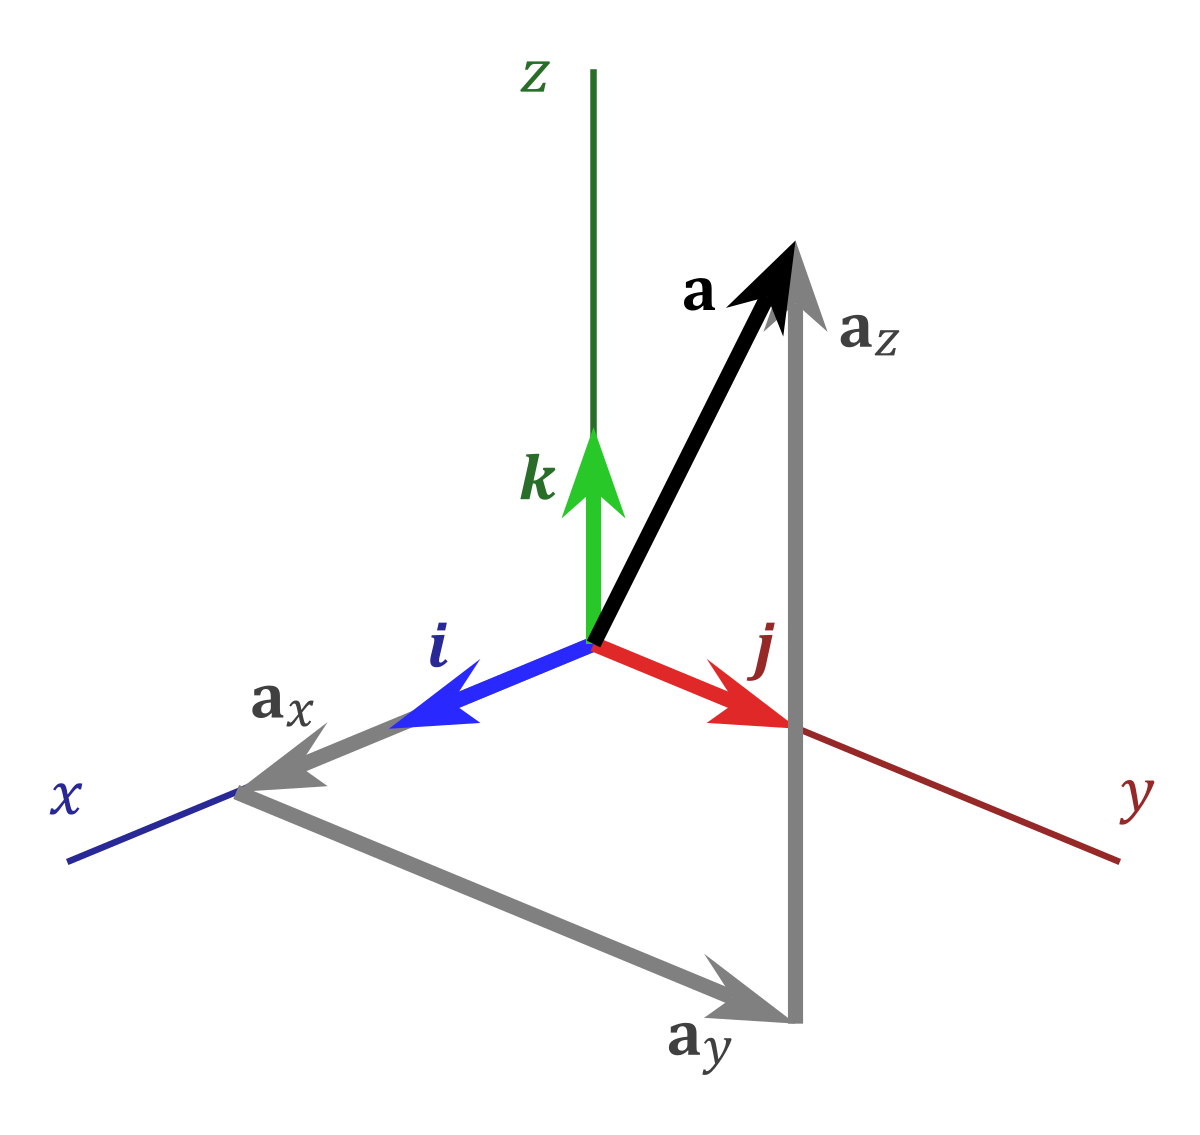
\includegraphics[width=.4\textwidth]{standardbasis}
		
		{\footnotesize Standard basis vectors in $\mb{R}^3$: $\bm{i, j, k}$ or
			$\bm{e_1, e_2, e_3}$. 
			
			Source: \url{https://en.wikipedia.org/wiki/Standard_basis}}
		
	\end{center}
\end{frame}

\begin{frame}
  \frametitle{Vector norms}
  \pause
  Norm of a vector (p-norm) \pause
    \begin{equation}
      ||\bm x||_{D} = \lt(\sum_{n} |x_{n}|^{D}\rt)^{\fr1D}
    \end{equation}

    \pause
  \begin{itemize}
  \item Euclidean, $\ell^2$, or 2-norm:
    \pause
    \begin{equation}
      ||\bm x||_2 = \sqrt{\sum_{n=1}^N x_n^2}
    \end{equation}
    \pause           
    $||\bm x||_2^2 = \bm x\tr \bm x$
    \pause
  \item $\ell^1$ or 1-norm:\pause
    \begin{equation}
      ||\bm x||_1 = \sum_{n=1}^N |x_n|
    \end{equation}
    \pause
  \item Max-norm:\pause
    \begin{equation}
      ||\bm x ||_\infty = \max_n|x_n|
    \end{equation}


  \item Unit vector: one whose Euclidean norm is 1: \pause $||\bm x||_{2} =1$
    \pause

  \end{itemize}
\end{frame}
\begin{frame}
	\frametitle{Special vectors}
	\pause
	
	\begin{itemize}
		\item  The vector of ones: $\bm 1$.
		\pause
		
		\item Vector of zeros: $\bm 0$.
		
		\pause
		
		\item Unit (or one-hot) vector: all zeros except for entry $i$ with
		a value of 1.\pause
		\begin{equation}
			\bm e_4 \in \mb{R}^5 = (0,0,0,1,0)
		\end{equation}
	\end{itemize}
\end{frame}


\section{Matrices}
\begin{frame}
	\frametitle{Transpose and trace}
	\pause
	\begin{itemize}
		\pause
		
		\item The transpose $\bm A\tr$of a matrix $\bm A$ is obtained by
		converting row elements to column elements and vice versa: \pause
		\begin{equation}
			[\bm A\tr]_{ij} = [\bm A]_{ji}
		\end{equation}
		\pause
		If $\bm A$ is an $n\times p$ matrix, then $\bm A\tr$ is $p \times n$.
		\pause
		
		\item A matrix $\bm A\in\mb{R}^{n\times p}$ is \textbf{square} if $n=p$.
		
		\pause 
		
		\item If a square matrix $\bm A$ is equal to it transpose ($\bm A =
		\bm A\tr$), then $\bm A$ is \textbf{symmetric}.
		
		\item The trace $\text{tr}(\bm A)$ of a square matrix $\bm A$ is the sum of its diagonal elements:\pause
		\begin{equation}
			\text{tr}(\bm A) = \sum_{i=1}^{n}a_{ii}
		\end{equation}
		
	\end{itemize}
\end{frame}

\begin{frame}
  \frametitle{Matrix norms}
  \pause
  Given a matrix $\bm A\in\mb{R}^{M\times N}$ defining a function
  $f(\bm x) = \bm A\bm x$, the \textbf{induced p-norm} of $\bm A$ is
  given by:\pause

  \begin{equation}
    ||\bm A||_D = \max_{||\bm x||=1}||\bm A\bm x||_D
  \end{equation}

  \pause

  For $D=2$:\pause
  \begin{equation}
    ||\bm A||_2 = \sqrt{\la_{\max}(\bm A\tr\bm A) } = \max_n\si_n
  \end{equation}
  \pause
  where $\la_{\max}$ is the greatest eigenvalue and $\si_n$ is $n$-th
  singular value.

\end{frame}


\begin{frame}
  \frametitle{Determinants}
  \pause

  Geometrically, the determinant, det$(\bm A)$ or $|\bm A|$, of a square
  matrix is the [directional] scaling factor of a unit area/volume
  transformed by the matrix. \pause

  \begin{itemize}
  \item If $\bm A =
    \begin{pmatrix}
      a & b \\ c & d
    \end{pmatrix}$, then:
    \pause
    \begin{equation}
      |\bm A| = ad - bc
    \end{equation}
    \pause
  \item The determinant of a singular (noninvertible) matrix is 0.
    \pause
  \item The determinant of matrix is equal to the product of its
    eigenvalues:
\pause
\begin{equation}
  |\bm A| = \prod_{i=1}^n \la_i
\end{equation}
  \end{itemize}
\end{frame}



\begin{frame}
  \frametitle{Range and nullspace}
  \pause

  The range (column space) of a matrix $\bm A\in \mb{R}^{m\times n}$ is the set of all the vectors that can be
  expressed as a linear combination of the column vectors of $\bm A$.
\pause

\begin{equation}
  \text{range}(\bm A) := \pause \{\bm v \in \mb{R}^m: \bm v = \bm A\bm
  x, \bm x \in \mb{R}^n\}
\end{equation}

\pause

The nullspace of a matrix is the set of all vectors $\bm v$ such that
$\bm A\bm v = \bm 0$: \pause
\begin{equation}
  \text{nullspace}(\bm A) := \pause \{\bm v \in \mb{R}^n: \bm A\bm v =
  \bm 0\}
\end{equation}

\end{frame}

\begin{frame}
  \frametitle{Rank}
  \pause The rank of a matrix is the greatest number of its LI column
  vectors (or row vectors) \pause
\begin{itemize}
\item This is equivalent to the dimension of the vector space spanned
  by its columns (or by its rows)
  \pause
\item Given $\bm A\in\mb{R}^{m\times n}$:
  \begin{equation}
    \text{rank}(\bm A) \le \min(m,n)
  \end{equation}
\pause
\item A matrix $\bm A\in\mb{R}^{m\times n}$ is full rank if
  $\text{rank}(\bm A) = \min(m,n)$.

\pause

\item Any matrix that is not full rank is \textbf{rank deficient}
\pause

\item A square matrix is invertible if and only if it is full rank
\pause

\item $\text{rank}(\bm A) = \text{rank}(\bm A\tr) = \text{rank}(\bm
  A\tr\bm A) = \text{rank}(\bm A\bm A\tr)$

\end{itemize}
\end{frame}

\begin{frame}
	\frametitle{Condition number}\pause
	The condition number $\kappa$ of a matrix measures how numerically stable it is under computation: \pause
	
	\begin{equation}
		\kappa (\bm A)  = ||\bm A|| \cdot ||\bm A^{-1}||
	\end{equation}
	\pause
	where $||\bm A||$ is typically taken as the $\ell_2$ norm of $\bm A$.
	\pause
	
	\begin{itemize}
		\item $\bm A$ is well-conditioned when $\kappa (\bm A)$ is close to 1
		\item $\bm A$ is ill-conditioned when $\kappa (\bm A)$ is large (nearly singular/noninvertible)
	\end{itemize}
\end{frame}

\section{Special matrices}
\begin{frame}
	\frametitle{Special matrices}
	\pause
	
	\begin{itemize}
		\item \textbf{Diagonal matrix:} square matrix; all elements 0 except on the main diagonal
		\pause
		\begin{equation*}
			\bm A = \text{diag}(\bm a) = \pause
			\begin{bmatrix}
				a_{1} & 0 & \cdots & 0 \\
				0 & a_{2} & \cdots & 0 \\
				\vdots & \vdots & \ddots & \vdots \\
				0 & 0  & \cdots & a_{n} \\        
			\end{bmatrix}
		\end{equation*}
		
		\pause
		\item \textbf{Identity matrix:} diagonal matrix whose non-zero elements are 1 \pause
		
		\begin{equation*}
			\bm I_{n} =
			\begin{bmatrix}
				1 & 0 & \cdots & 0 \\
				0 & 1 & \cdots & 0 \\
				\vdots & \vdots & \ddots & \vdots \\
				0 & 0  & \cdots & 1 \\         
			\end{bmatrix}_{n\times n}
		\end{equation*}
		\pause
		
		\item \textbf{Block diagonal matrix:} concatenates matrices onto the main diagonal of a single one
		\pause
		\begin{equation*}
			\bm Z = \pause
			\text{blkdiag}(\bm A, \bm B, \bm C) = \pause
			\begin{bmatrix}
				\bm A & \bm 0 & \bm 0 \\
				\bm 0 & \bm B & \bm 0 \\
				\bm 0 & \bm 0 & \bm C
			\end{bmatrix}
		\end{equation*}
	\end{itemize}
\end{frame}

\begin{frame}
	\frametitle{Triangular matrices}
	\pause
	\begin{itemize}
		\item Upper triangular matrix: all non-zero entries are either on or
		above the diagonal:\pause
		\begin{equation*}
			\begin{pmatrix}
				1 & 4 & 7 & -2 \\
				0 & -3 & 1 & 10 \\
				0 & 0  & 7 & 2 \\
				0 & 0 & 0 & -1
			\end{pmatrix}
		\end{equation*}
		\pause
		\item Lower triangular matrix: all non-zero entries are either on or
		below the diagonal: \pause
		\begin{equation*}
			\begin{pmatrix}
				3 & 0 & 0 \\
				-1 & -2 & 0 \\
				9 & 4 & 1
			\end{pmatrix}
		\end{equation*}
		\pause
		\item The diagonal elements $A_{ii}$ of a triangular matrix $\bm A$
		are its eigenvalues.
	\end{itemize}
\end{frame}

\begin{frame}
	\frametitle{Positive definite matrices}
	\pause
	Given a symmetric matrix $\bm A \in \mb{S}^n$ and a non-zero vector
	$\bm x \in \mb{R}^n$, $\bm A$ is:
	\pause
	
	\begin{itemize}
		\item positive definite if $\forall \bm x$: $\bm x\tr\bm A\bm x > 0$
		\pause
		\item positive semidefinite (psd) if $\forall \bm x$: $\bm x\tr\bm A\bm x
		\ge 0$
		\pause
		\item negative definite if $\forall \bm x$: $\bm x\tr\bm A\bm x < 0$
		\pause
		\item negative semidefinite if $\forall \bm x$: $\bm x\tr\bm A\bm x
		\le 0$
		\pause
		\item indefinite if neither psd nor nsd\pause
		\item \textbf{Gram matrix} $\bm G$ is always psd: \pause
		\begin{equation}
			\bm G = \bm X\tr\bm X 
		\end{equation}
		given any matrix $\bm X\in\mb{R}^{m\times n}$
	\end{itemize}
\end{frame}

\begin{frame}
	\frametitle{Orthogonal matrix}
	
	\pause
	
	\begin{itemize}
		\item Two vectors $\bm x,\bm y\in\mb{R}^n$ are orthogonal if $\bm
		x\tr \bm y = 0$. \pause
		
		\item A normalized vector is one whose 2-norm is 1. \pause
		
		\item Thus, a set of vectors that is pairwise orthogonal and
		normalized is \textbf{orthonormal}
		\pause
		\item A square matrix $\bm U\in\mb{R}^{n\times n}$ is
		\textbf{orthogonal} if all its columns are orthonormal
		\pause
		
		\item The inverse of $\bm U$ is its transpose: \pause
		\begin{equation}
			\bm U\tr\bm{U}= \pause \bm U\bm U\tr  = \bm I 
		\end{equation}
		\pause which implies: $\bm U^{-1} = \bm U\tr$
	\end{itemize}
	
	
\end{frame}

\begin{frame}
  \frametitle{Nonsingular matrices}
  \pause

  A matrix is nonsingular (invertible) only if it is square and if its columns are  linearly independent.

  \pause

  The inverse of a matrix $\bm X$ is given by $\bm X^{-1}$ and
  satisfies the property:\pause
 \begin{equation}
    \bm X^{-1}\bm X = \bm X \bm X^{-1} = \bm I_{n}
  \end{equation}
  
\pause

\begin{itemize}
\item $\bm X^{-1}$ exists $\iff |\bm X| \ne 0$ \pause
\item $(\bm X^{-1})^{-1} = \bm X$ \pause
\item $(\bm W\bm X)^{-1} = \bm X^{-1}\bm W^{-1}$ \pause
\item For 2D case:\pause
  \begin{equation}
    \bm A =
    \begin{pmatrix}
      a & b\\ c& d
    \end{pmatrix},\quad\pause \bm{A}^{-1} = \fr1{|\bm A|}
    \begin{pmatrix}
      d & -b \\ -c & a
    \end{pmatrix}
  \end{equation}

\pause
\item For block diagonal matrix:\pause
  \begin{equation}
    \begin{pmatrix}
      \bm A & \bm 0 \\ \bm 0 & \bm B
    \end{pmatrix}^{-1}
 =
 \begin{pmatrix}
   \bm A^{-1} & \bm 0 \\ \bm 0 & \bm B^{-1}
 \end{pmatrix}
  \end{equation}

\end{itemize}
\end{frame}




\begin{frame}
  \frametitle{Other important results}
  \pause

  Read \textbf{PMLI} 7.3 for details

  \begin{itemize}
  \item Schur complement: \pause
  Given  a partitioned matrix $\bm M = \begin{pmatrix}
  	\bm E & \bm F \\ \bm G & \bm H
  \end{pmatrix}$ then:
  
  \begin{align}
  	\bm M/\bm H &= \bm E - \bm F\bm H^{-1} \bm G \quad \text{(Schur complement of $\bm M$ wrt $\bm H$)} \\
  	\bm M/\bm E &= \bm H - \bm G\bm E^{-1} \bm F
  \end{align}
  \item Matrix inversion lemma (Sherman-Morrison formula)
  \item Matrix determinant lemma:
    \begin{equation}
      |\bm A + \bm u\bm v\tr| = (1 + \bm v\tr\bm{A}^{-1})\bm u|\bm A|
    \end{equation}
  \end{itemize}
\end{frame}
  
\section{EVD}

\begin{frame}
  \frametitle{Eigenvectors and eigenvalues (review)}
  A vector $\bm v$ is an eigenvector of a matrix $A$ if its transformation by $A$ scales rather than changes the direction of $\bm v$:\pause
  \begin{equation}
    \label{eq:5}
    \bm A \bm v = \pause \la \bm v
  \end{equation}\pause
  where $\la$ is the \textbf{eigenvalue} (a scalar).
\pause
  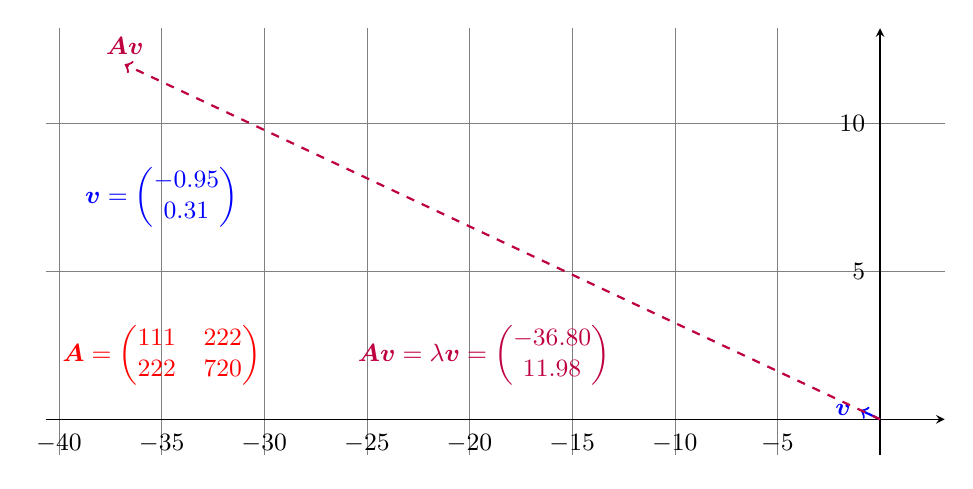
\begin{tikzpicture}[]\small
    \begin{axis}[no markers, domain=-40:0, %samples=100,
      axis x line=center,
      axis y line=center,
      %xlabel=$z$, ylabel=$f_X(x)$,,
      height=7cm, width=13cm,
      % xtick={-6,0,6},
      % xticklabels={$z_{\alpha/2}$,$0$,$z_{(1-\alpha/2)}$},
      ymax=12,ymin=0,xmax=-0.5, xmin=-37,
      % ytick=\empty,
      % x label style={anchor=west},
      % y label style={anchor=south},
      %
      enlargelimits=true, clip=false, %axis on top,
      grid style={line width=.1pt, draw=gray},
      % yticklabel style={
      % /pgf/number format/fixed,
      % /pgf/number format/fixed zerofill,
      % /pgf/number format/precision=2
      % },        
      grid = both
      ]
      \visible<+->{
        \draw[->, thick, blue] (axis cs: 0,0) -- (axis cs:  -0.95, 0.31) node[left] {$\bm v$};
      \node[blue] (a) at (axis cs: -35, 7.5) {\small$\bm v =
        \begin{pmatrix}
          -0.95 \\ 0.31
        \end{pmatrix}
        $};        
    }
      \visible<+->{
      \node[red,below=of a] (b) {\small$\bm A =
        \begin{pmatrix}
          111 & 222 \\
          222 & 720
        \end{pmatrix}
        $} ;}
    \visible<+->{
      \draw[->, thick, dashed, purple] (axis cs:  0,0) -- (axis cs: -36.8, 11.98) node[above] {$\bm{Av}$};
      \node[purple, right=of b] (c) {\small$\bm {Av} = \la \bm v =
        \begin{pmatrix}
          -36.80 \\ 11.98
        \end{pmatrix}
        $};
    }
  \end{axis}
  \end{tikzpicture}
\end{frame}



\begin{frame}
  \frametitle{Eigenvalue-related properties}
  \pause
  \begin{itemize}
  \item The solutions of the characteristic equation\pause
    \begin{equation}
      \text{det}(\la\bm I - \bm A)\bm v = \bm 0,\quad \bm v\ne \bm 0
    \end{equation}
    are the eigenvalues $\la_i$ of $\bm A$.
    \pause
  \item The trace of a matrix is the sum of its eigenvalues \pause
  \begin{equation}
  	\text{tr}(\bm A) = \sum_{i=1}^n \la_i
  \end{equation}
\pause

\item The determinant of a matrix is the product of its eigenvalues \pause
\begin{equation}
	\text{det}(\bm A) = \prod_{i=1}^n \la_i
\end{equation}
\pause
\item The rank of a matrix is equal to the number of its non-zero eigenvalues
  \end{itemize}

\end{frame}

\begin{frame}
  \frametitle{Eigenvalue decomposition (EVD)}
  \pause

  We can write: \pause
  \begin{equation}
    \bm A\bm U = \bm U \bm A
  \end{equation}
\pause
where the columns of $\bm U \in \mb{R}^{n\times n}$ are the
eigenvectors of $\bm A$ \pause
\begin{equation}
  \bm U \in \mb{R}^{n\times n} =
  \begin{pmatrix}
    \mid & \mid &  & \mid \\
    \bm u_1 &\bm u_2 & \ldots & \bm u_n \\
    \mid & \mid &  & \mid \\
  \end{pmatrix}
\end{equation}

\pause
and $\bm\Lambda$ is a diagonal matrix of the
eigenvalues:
\pause
\begin{equation}
  \bm\Lambda = \text{diag}(\la_1,\ldots, \la_n)
\end{equation}
\pause
\begin{itemize}
\item $\bm A$ is said to be diagonalizable \pause

\item EVD: If $\bm U$ is invertible, then we can also write: \pause
  \begin{equation}
    \bm A = \bm U\bm\Lambda\bm U^{-1}
  \end{equation}
\end{itemize}
\end{frame}

\begin{frame}
  \frametitle{Symmetric matrices}
  \pause
  When $\bm A$ is real and symmetric, then $\bm U$ is orthogonal:\pause
  \begin{equation}
      \bm A = \bm U\bm\Lambda\bm U^{-1} = \bm U\bm\Lambda\bm U\tr
      \pause = \sum_{i=1}^n\la_i\bm u_i\bm u_i\tr
  \end{equation}
\pause
And
\begin{equation}
  \bm A^{-1} = \bm U\bm\Lambda^{-1}\bm U\tr = \pause
  \sum_{i=1}^d\fr{1}{\la_i} \bm u_i\bm u_i\tr
\end{equation}
\end{frame}
\begin{frame}
  \frametitle{Singular value decomposition (SVD)}
  The singular value decomposition of $\bm X$ generalizes EVD to
  rectangular matrices:

  \begin{equation}
    {\bl \bm X} = \bm {{\rd U}{\gr \Gamma} {\pl V}}^T 
  \end{equation}

  \pause

  where:
  \begin{itemize}[<+->]
  \item   $\bm X$ is an $n\times p$ data matrix
%, whose entries have been centered ($x_{ij} \leftarrow x_{ij} - \ol{x}_j$)
  \item $\bm U$ is an $n\times p$ orthogonal\footnote{i.e.\ $\bm U^T\bm U = \bm I$ and $\bm U^T = \bm U^{-1}$} matrix. The columns of $\bm U$ are called \textit{\rd left singular vectors}
  \item  $\bm \Gamma$ is a $p\times p$ diagonal matrix (whose elements are called \textit{\gr singular values})
  \item  $\bm V$ is an $p\times p$ orthogonal\footnote{i.e.\ $\bm V^T\bm V= \bm I$  and  $\bm V^T = \bm V^{-1}$} matrix. The columns of $\bm V$ are called \textit{\pl right singular vectors}
  \item The columns of $\bm{U\Gamma}$ are called the \textbf{principal components} of $\bm X$.
\end{itemize}

\end{frame}

\begin{frame}
  \frametitle{SVD (cont.)}

  \begin{eqnarray*}\pause
    \bl
  \overbrace{
    \begin{pmatrix}
      x_{11}   & \cdots & x_{1p} \\
      \vdots  & \ddots & \vdots \\
      x_{n1}   & \cdots & x_{np} 
    \end{pmatrix}
  }^{\bm X}
  &=&\pause
{\rd  \overbrace{\begin{pmatrix}
      u_{11}  & \cdots & u_{1p} \\
       \vdots  & \ddots & \vdots \\
      u_{n1}   & \cdots & u_{np}     
    \end{pmatrix}}^{\bm U: \text{ eigenvectors of } \bm{XX}^T}} \pause
  {\gr \overbrace{
    \begin{pmatrix}
      \sqrt{\la_1}              & \cdots & 0 \\
       0                       & \ddots & 0 \\
       0                       & \cdots & \sqrt{\la_p}
    \end{pmatrix}
  }^{\substack{\bm\Gamma: \text{ $\sqrt{\text{eigenvalues}}$ of $\bm{XX}^T$ }  \\ \text{also singular values of } \bm X }}} \pause
{\pl \overbrace{\begin{pmatrix}
      v_{11}   & \cdots & v_{1p} \\
       \vdots  & \ddots & \vdots \\
      v_{p1}   & \cdots & v_{pp}     
    \end{pmatrix}}^{\bm V: \text{ eigenvectors of } \bm{X}^T\bm X}  
}  \end{eqnarray*}

  \pause

  \begin{itemize}[<+->]
  \item The columns $\rd \bm u_1, \ldots, \bm u_p$ are the left singular vectors of $\bm X$
  \item  The columns $\pl \bm v_1, \ldots, \bm v_p$ are the right singular vectors of $\bm X$
  \item The elements $\gr \sqrt{\la_1} \ge \ldots \ge  \sqrt{\la_p} = 0$ are the singular values of $\bm X$
  \item $\la_1\ge  \ldots \ge \la_p =0$ are the eigenvalues of $\bm {XX}^T$ and also of $\bm X^T \bm X$
  \end{itemize}
\end{frame}


\section{Linear systems}
\begin{frame}
  \frametitle{Solving a system of equations}
  \pause
  A system of linear equations can be represented and solved as
  follows: \pause
  \begin{eqnarray*}
    \bm{Ax} &=& \bm b \\\pause
    \bm{A}^{-1}\bm{Ax} \pause &=& \bm A^{-1}  \bm b \\
    \bm I_{n}\bm x &=& \bm A^{-1}\bm b \\
    \bm x &=& \bm{A}^{-1}\bm b
  \end{eqnarray*}
\pause
\begin{itemize}
\item  If $\bm A\in\mb{R}^{m\times n}$, then there are $m$ equations
  and $n$ unknowns \pause
\item If $m=n$, then $\bm A$ is full rank, and there is a unique
  solution \pause

\item If $m < n$, the system is \textbf{underdetermined} (no unique
  solution)

\item If $m>n$, the system is \textbf{overdetermined} (no exact
  solution; solve via least squares)
\end{itemize}
\end{frame}

\begin{frame}
  \frametitle{Least squares}
  \pause
  Given a system $\bm A\bm x = \bm b$, the least squares objective is:
  \pause
  \begin{equation}
    \min_{\bm x} f(\bm x) \equiv \min_{\bm x} \fr12||\bm A\bm x - \bm b||_2^2
  \end{equation}
  \pause
  The gradient is given by:\pause
  \begin{equation}
    \bm g(\bm x) = \fr{\partial}{\partial \bm x} f(\bm x) = \bm A\tr\bm A\bm x - \bm
    A\tr\bm b
  \end{equation}
  \pause
  The optimal $\bm {\hat x}$ is found by solving for $\bm g(\bm x) =
  \bm 0$: \pause
  \begin{equation}
     \bm{A}\tr\bm A\bm x = \bm  A\tr\bm b
  \end{equation}
  \pause
  And thus,
  \begin{equation}
    \hat{\bm x} = ( \bm A\tr\bm A)^{-1}\bm A\tr \bm b
  \end{equation}
  \pause 
  is the ordinary least squares (OLS) solution.
\pause
Checking that the Hessian $\bm H(\bm x) = \bm A\tr\bm A$ is pd
confirms the solution is unique.
\end{frame}

\section{Outlook}

\begin{frame}
  \frametitle{Reading assignments}

  \begin{itemize}
  \item \textbf{PMLI} 7
  \item \textbf{PMLCE} 2
  \end{itemize}
\end{frame}

% \begin{frame}
%   \frametitle{Introduction to Python/JupyterLab/R}
%   \pause

%   More will be said on this next lecture.

%   \pause

%   You can find a helpful tutorial at \url{https://cs231n.github.io/python-numpy-tutorial/#jupyter-and-colab-notebooks}.
% \end{frame}


\end{document}

%%% Local Variables:
%%% mode: latex
%%% TeX-master: t
%%% End:
